\def\year{2015}
%File: formatting-instruction.tex
\documentclass[letterpaper]{article}
\usepackage{aaai}
\usepackage{times}
\usepackage{helvet}
\usepackage{courier}
\usepackage{color}
\usepackage{algorithm}
\usepackage{algorithmic}
\frenchspacing
\setlength{\pdfpagewidth}{8.5in}
\setlength{\pdfpageheight}{11in}
\pdfinfo{
/Title (Insert Your Title Here)
/Author (Put All Your Authors Here, Separated by Commas)}
\setcounter{secnumdepth}{0}
\usepackage{amsmath}  
\usepackage{amsfonts}
\DeclareMathOperator*{\argmin}{\arg\!\min} 
\DeclareMathOperator*{\argmax}{\arg\!\max} 
\usepackage{graphicx}
\usepackage{mathtools}
\newif\ifnotes
%\usepackage{natbib}

%---------Toggle these flags if you want to supress the comments------------
\notestrue
%\notesfalse
%-----------------------------------------------------------------------------

\newcommand{\citet}[1]{\citeauthor{#1}~(\citeyear{#1})}

\ifnotes
\newcommand{\sw}[1]{\textcolor{red}{SW: #1}}
\newcommand{\jm}[1]{\textcolor{blue}{Joao: #1}}
\newcommand{\ks}[1]{\textcolor{green}{Kyriacos: #1}}
\else
\newcommand{\sw}[1]{}
\newcommand{\jm}[1]{}
\newcommand{\ks}[1]{}
\fi

 \begin{document}
% The file aaai.sty is the style file for AAAI Press 
% proceedings, working notes, and technical reports.
%
\title{Inverse Reinforcement Learning from Failure}
% \author{AAAI Press\\
% Association for the Advancement of Artificial Intelligence\\
% 2275 East Bayshore Road, Suite 160\\
% Palo Alto, California 94303\\
% }
\maketitle
\begin{abstract}
\begin{quote}

\emph{Inverse reinforcement learning} (IRL) allows autonomous agents to learn to solve complex tasks from successful demonstrations.  However, in many settings, e.g., when a human learns the task by trial and error, \emph{failed} demonstrations are readily available.  In addition, in some tasks, purposely generating failed demonstrations may be easier than generating successful ones.  Since existing IRL methods cannot make use of failed demonstrations, in this paper we propose \emph{inverse reinforcement learning from failure} (IRLF)\emph{inverse reinforcement learning from failure} (IRLF) which exploits both successful and failed demonstrations.  Starting from the state-of-the-art \emph{maximum causal entropy IRL} method, we propose a new constrained optimisation formulation that accomodates both types of demonstrations while remaining convex.  We then derive update rules for learning reward functions and policies. Experiments on both simulated and real-robot data demonstrate that IRLF converges faster and generalises better than maximum causal entropy IRL, especially when few successful demonstrations are available.

\end{quote}
\end{abstract}

\section{Introduction}
Inverse Reinforcement Learning (IRL) \cite{ng2000algorithms} %along with the closely related field of Inverse Optimal Control (IOC)
methods address the problem of learning reward functions for decision making tasks from human demonstration. IRL methods are especially applicable to complex tasks where the desired behavior can be easily demonstrated, but in which an appropriate reward function is hard to formalise \emph{a priori}. The learned reward function attempts to encode the relative preferences and goals of the human controller, and can be used to induce control policies for reward-seeking autonomous agents that imitate the demonstrated behavior. Learning a reward function, as opposed to learning directly a control policy, also makes it easier to generalize the desired behavior to other similar domains.

All Inverse Reinforcement Learning methods to date focus on the imitation of a certain type of behaviour, which is presented to the learning algorithm as a set of \emph{successful} demonstrations of how to solve the given task. However, there are tasks for which we might have data that demonstrates behaviour that we would like to avoid. This may occur, for instance, in complex tasks that a human controller learns to solve through trial and error, and where demonstrations of both successful and failed behaviour are available. %, and labeling them as such is straightforward. 
\jm{Maybe a couple of motivating examples if there's space?}. Currently existing IRL methods do not provide any means of leveraging the failed demonstrations, even though that data also contains information regarding the behavior that the learner agent should \emph{not} perform in certain situations, which could also be expressed in the learned reward function, and that could help in generalising the desired behavior to other domains or problem conditions.

For some tasks, demonstrating the behaviour to be avoided may even be easier than demonstrating successful behaviour, which could require great expertise. If that behaviour is dangerous or otherwise undesireable to demonstrate in a real system, it could be simulated, and the respective examples could be used to learn to avoid the undesired behaviour in the real world. %Finally, learning to avoid behaviours could be useful in Active and Lifelong Learning since a human would be able to specify behaviours of the agent that are undesirable at the trajectory level (instead of the action level). 

Inverse Reinforcement Learning was introduced by \cite{ng2000algorithms} and \cite{abbeel2004apprenticeship}. The first probabilistic interpretation of the framework was introduced by \citet{ramachandran2007bayesian} and extended to Maximum Entropy IRL by \citet{ziebart2008maximum}. Learning from failure is an area that has found most attention in the Robotics community, specifically in imitation learning. \cite{choi2015} introduces leveraged non stationary Gaussian processes, that fit good data points while trying to avoid bad examples. The method was also applied to robotic navigation, but not in terms of IRL. \cite{grollman2012robot} use past failures of the robot to initialise robot policies, and conclude that there is indeed information in failed trajectories that should not be discarded. %IRL has been previously applied to social robot navigation. Notable works are those of \cite{henry2010learning} and \cite{vasquez2014inverse}, that use pedestrian simulators to extract the underlying reward function of a human controller. 

In this paper, we introduce \emph{inverse reinforcement learning from failure} (IRLF), which is to our knowledge the first IRL algorithm that can learn useful reward functions from both successful and failed demonstrations. Starting from Maximum Causal Entropy IRL \cite{ziebart2010modelingthesis}, we first present the modifications to the optimization problem that allow the incorporation of failed demonstrations into the learning process, while ensuring that the problem remains convex. Then, we derive the update rules to learn a policy and its respective reward function while taking into account both the successful and the failed examples.

We evaluate our algorithm on simulated and real-robot data, in the context of learning social navigation for a mobile robot. On the simulated scenarios, our results demonstrate IRLF's ability to generalise better in the presense of limited successful examples with little extra computational cost. Finally, on real robotic navigation data the algorithm yields consistently superior results when compared to the state-of-the art \sw{vague: give specifics about performance} \jm{Will need to be revised with the actual final results that we get}. \jm{I omitted an argument that the algorithm is able to learn ``mixtures of behaviors'' from successful and failed examples, since that is quite difficult to fit in here without raising too much confusion} 


\section{Background}
Most IRL methods formalize the underlying decision-making problem as a \emph{Markov decision process} (MDP), a model of a discrete-time process wherein an agent's actions may stochastically influence its environment. In an MDP, at step $t$, the system (which includes the agent and its environment) is known to be in a \emph{state} $s_t\in\mathcal{S}$; the agent selects an action $a_t\in\mathcal{A}$ and is awarded a real-valued \emph{reward}; and the system jumps to state $s_{t+1}$ with probability $P(s_{t+1}|s_t,a_t)$. Formally, an MDP is a tuple $\langle\mathcal{S},\mathcal{A},T,R\rangle$, where $\mathcal{S}$ and $\mathcal{A}$ are sets of discrete states and actions respectively, $T:\mathcal{S}\times\mathcal{A}\times\mathcal{S}\rightarrow [0,1]$ is a transition function such that $T(s,a,s')=P(s'|s,a)$, and $R:\mathcal{S}\times\mathcal{A}\rightarrow\mathbb R$ is the reward function. 
Optimally solving an MDP involves finding a policy $\pi:\mathcal{S}\times\mathcal{A}\rightarrow[0,1]$ with $\pi(s,a) = P(a\,|\,s)$, which maximises the expected sum of rewards over a fixed number of decisions $h$. This expectation can be expressed as the \emph{value} of policy $\pi$:
\begin{equation}
\label{eq:value}
 V^\pi(s) \coloneqq E\{\sum_{t = 1}^hR(s_t,a_t)\,\vert\, s_1 = s\}.
\end{equation}

Given data obtained from interacting with an MDP, RL methods seek a policy that maximizes this expectation for a given reward function.  By contrast, given data obtained from \emph{expert} interactions wtih an MDP, IRL seeks the reward function that the expert was maximizing.  IRL is useful in the many situations in which the expert cannot easily formalize her objectives as a reward function.  Instead, the \emph{learner}, a reward-seeking autonomous agent, can learn the reward function from the expert's behavior and use it to imitate her.

IRL is formalized as an `incomplete' MDP $\langle\mathcal{S},\mathcal{A},T\rangle$, also known as an MDP/R. Though initially unknown, the reward function is parametrized by $K$ \emph{feature functions}, $\phi_k(s,a)$:
\begin{equation}
R(s,a) = \sum_{k=1}^Kw_k\phi_k(s,a), \label{eq:rew}
\end{equation}
where $w=[w_1\,w_2\,\ldots\,w_k]^T$ is the weight vector that IRL aims to learn.

Since $w$ is independent of states and actions, \eqref{eq:value} and \eqref{eq:rew} imply a parametric form of the value function:
\begin{align}
 	V^{\pi}(s) &= \sum^K_{k=1}w_k\left(E\{\sum_{t = 1}^h\phi_k(s_t,a_t)\,\vert\, s_1 = s\}\right)\\
&\eqqcolon\sum^K_{k=1}w_k\mu^{\pi, 1:h}_k|_{s_1=s},\label{eq:parametrized_value}
\end{align}
where $\mu^{\pi,1:h}_k|_{s_1=s}$, the \emph{feature expectation}, is the expected accumulated instances of feature $\phi_k$ between steps $1$ and $h$ under policy $\pi$  given that $s_1 = s$.

The learner learns from $\mathcal{D} = \big\{ \tau_1,\tau_2,...\tau_N \big\}$, a dataset of $N$ trajectories. Each trajectory $\tau_i = \left<(s^{\tau_i}_1,a^{\tau_i}_1),(s^{\tau_i}_2,a^{\tau_i}_2),\ldots,(s^{\tau_i}_{h},a^{\tau_i}_{h})\right>$ is a state-action sequence of length $h$ generated by the expert.

Given $\mathcal{D}$, the learner can compute the \emph{empirical feature expectation}, the accumulated instances of each feature in $\mathcal{D}$:
\begin{equation}
	\widetilde{\mu}^{\mathcal{D}}_k \coloneqq\frac{1}{N}\sum_{\tau\in\mathcal{D}}\sum_{t=1}^{h}\phi_k(s^\tau_t,a^\tau_t). \label{eqn:empirical_fe}
\end{equation}
Note that $\widetilde{\mu}^{\mathcal{D}}_k$ is state independent and implicitly estimates an expectation across
the expert's initial state.  To fairly compare the feature expectation of some policy $\pi$ to $\widetilde{\mu}^{\mathcal{D}}_k$, we obtain an analogously state-independent measure of $\pi$'s feature expectation by marginalising out $s_1$:
\begin{align}
  \label{eq:feature_expectation_belief}
  \mu^{\pi,1:h}_k \coloneqq \sum_{s\in\mathcal{S}}P(s_1 = s)\mu^{\pi,1:h}_k|_{s_1=s},
\end{align}
where $P(s_1 = s)= N_1(s)/N$ is the maximum likelihood estimate of the expert's initial state distribution, given that $N_1(s)$ is the number of trajectories with $s_1 = s$.

The learner aims to find $w$ such that the distance between the vectors $\widetilde\mu^{\mathcal{D}}~=~[\widetilde\mu^{\mathcal{D}}_1\,\ldots\,\widetilde\mu^{\mathcal{D}}_k]^T$ and $\mu^{\pi}~=~[\mu^{\pi}_1\,\ldots\,\mu^{\pi}_k]$ is minimized according to some metric, while also generalising well to unseen initial conditions.

IRL methods are typically iterative. An initial guess for $w$ is fed to a planner that produces a policy $\pi$ that is optimal given $w$.  Using $\pi$, trajectories are generated from the same initial states as in $\mathcal{D}$ to compute $\mu^{\pi}$, which is then compared to $\widetilde{\mu}^{\mathcal{D}}$.  Finally, $w$ is updated to reduce to distance between the two, and the process repeats.

Existing IRL methods use structured prediction \cite{ratliff2006maximum}, Bayesian inference \cite{ramachandran2007bayesian}, Gaussian processes \cite{levine2011nonlinear}, neural networks and decision trees \cite{ratliff2007boosting} to learn $w$.  In this paper, we concentrate on two similar methods by \citet{ziebart2008maximum} and \citet{ziebart2010modelingthesis} that learn maximum-entropy policies.  A maximum-entropy approach is attractive because it is probabilistic and thus robust to noise and sub-optimal experts\jm{needs to be re-worded}, and results in convex optimisation problems. The methods work by solving the following constrained optimization problem:
\begin{align}
	\hbox{find:} &\quad\max\limits_{\pi(s,a)} H(\mathcal{A}^h||\mathcal{S}^h)\label{eq:primal_obj}\\
\hbox{subject to:}&\quad\widetilde{\mu}^{\mathcal{D}}_k   = \mu^{\pi}_k\quad\forall k \label{eq:features_equality_constraint}\\
\hbox{and:} &\quad\sum_{a\in\mathcal{A}}\pi(s,a)  = 1\quad\forall s\in\mathcal{S}\\
\hbox{and:} &\quad\pi(s,a) \geq 0\quad\forall s\in\mathcal{S},a\in\mathcal{A},  
\end{align}
where $H(\mathcal{A}^h||\mathcal{S}^h)$, the \emph{causal entropy}, is the conditional entropy of the action sequence $\mathcal{A}^h$, causally conditioned on the state sequence $\mathcal{S}^h$:
% For MDPs this quantity is fully determined given a policy $\pi$ and a transition function $T$:
\begin{align}
H(\mathcal{A}^h||\mathcal{S}^h) = -\sum_{t=1}^h \sum_{\substack{s_{1:t}\in\mathcal{S}^t\\a_{1:t}\in\mathcal{A}^t}} P(a_{1:t},s_{1:t})\log(P(a_t|s_t)),
\label{eg:entdef}
\end{align}
where:
\begin{align*}
  P(a_{1:t},s_{1:t})&= P(s_{1:t-1},a_{1:t-1})P(s_t|s_{t-1},a_{t-1})P(a_t|s_t)\\
  &=P(s_{t-1},a_{t-1})T(s_{t-1},a_{t-1},s_t)\pi(s_t,a_t).
\end{align*}
The contraints require that $\pi$ consists of proper probability distributions that match the empirical feature expectations.

The optimization problem is solved using the method of Lagrange multipliers. First, the equality constraint \eqref{eq:features_equality_constraint} is relaxed, yielding a Lagrangian:
\begin{equation}
\label{eq:partial_lagrangian}
\mathcal{L}(\pi,w)\coloneqq H(\mathcal{A}^h||\mathcal{S}^h) + \sum_{k=1}^Kw_k(\mu^{\pi}_k-\widetilde{\mu}^{\mathcal{D}}_k),
\end{equation}
and in turn a less constrained optimisation problem:
\begin{align}
\hbox{find:}\,\,&\,\,\min_{w}\left\{\max_\pi\left(\mathcal{L}(\pi,w)\right)\right\}\label{eq:partial_dual_obj}\\
\hbox{subject to:}\,\,&\sum_{a\in\mathcal{A}}\pi(s,a)  = 1\quad\forall s\in\mathcal{S}\label{eq:dual_constraint_1}\\
\hbox{and:}\,\,&\pi(s,a) \geq 0\quad\forall s\in\mathcal{S},a\in\mathcal{A},\label{eq:dual_constraint_2}
\end{align}

Differentiating $\mathcal{L}(\pi,w)$ with respect to $\pi$ at time $t$ results in \cite[p.\ 186]{ziebart2010modelingthesis}:
\begin{equation}
 \begin{split}
 &\nabla_{\pi(s_t,a_t)}\mathcal{L}(\pi,w) = P(s_{1:t},a_{1:t-1})\Bigg(-\log(\pi(a_t,s_t))+ \\
& H(\mathcal{A}^{t+1:h}||\mathcal{S}^{t+1:h})
 +\sum_{k=1}^K w_kE\left\{\sum_{\tau=1}^h \phi_k(s_t,a_t)|s_{1:t},a_{1:t-1}\right\}\Bigg). \label{eqn:zieb_lagragian_derivative}
 \end{split}
\end{equation}
Setting the gradient to zero and solving for $\pi$ gives:
\begin{equation}
\label{eq:policy_prop}
	\begin{split}
	&\pi(s_t,a_t) \propto \exp\left(H(\mathcal{A}^{t:h}||\mathcal{S}^{t:h})+\sum^K_{k=1} w_k\mu_k^{\pi,t:h}|_{s_t,a_t}\right).
	\end{split}
\end{equation}
Due to \eqref{eq:parametrized_value}, the rightmost term in \eqref{eq:policy_prop} is a measure of value for a given state and action, parametrized by $w$. \citet{ziebart2010modelingthesis} showed that solving \eqref{eq:policy_prop} while satisfying \eqref{eq:dual_constraint_1} and \eqref{eq:dual_constraint_2} amounts to solving a soft Bellman equation:
	\begin{equation}
		\begin{split}
	&Q_w(s,a)^{soft} = \sum_{k=1}^Kw_k\phi_k(s,a) + \sum_{s'}T(s,a,s')V_w(s'),\\	
	&V_w(s)^{soft} = \log\sum_{a}exp(Q_w(s,a)),\\
	&\pi(s,a) = \exp(Q_w(s,a) - V_w(s)).
	\end{split}
	\label{eq:soft_backup}
	\end{equation}
Once $\pi$ is computed for a given $w$, $w$ is itself updated via gradient descent, by noting that:
 \begin{align}
   \label{eq:weight_update}
   \nabla_{w}\mathcal{L}(\pi,w) =\mu^\pi - \mu^{\mathcal{D}}.
 \end{align}
The optimization process terminates once the weight vector converges to a local optimum. \sw{Why local? I thought it was convex.}

\section{Method}
	In this section we introduce a novel IRL algorithm that enables the incorporation of failed demonstrations into the learning process. We assume that these demonstrations come in the from of a second dataset $\mathcal{D}_f$ and in turn, produce empirical feature expectations that we define as $\widetilde{\mu}^{\mathcal{D}_f}$. As seen in equation \eqref{eq:parametrized_value}, the feature expectations have a direct relation to the Value of a policy. If therefore follows that we will now look for a weight vector, that will minimise the Value of the trajectories in this new dataset.
	In the original formulation[ref to eqs] the model was required to match the empirical expectations from succesful demonstrations ($\widetilde{\mu}^{\mathcal{D}}$). In addition to this requirement 
	our aim is to now learn a model that generates feature expectations that are dissimilar to the ones in the failed demonstrations. Although the failed demonstrations are semantically opposite to successfull ones, their incorporation into IRL proves to be non-trivial. In this section we describe a reliable and principled method of achieving just that.
	One way to express this additional requirement could be through additional inequality constraints in the optimisation problem,
	\begin{equation}
		\quad\widetilde{\mu}^{\mathcal{D}^f}_k  - \mu^{\pi}_k > \alpha_k \quad\forall k,
	\end{equation} 
	where $\alpha_k$ is a variable to be added to the optimisation objective.
	\begin{equation}
		\quad\max\limits_{\pi(s,a),\alpha} H(\mathcal{A}^h||\mathcal{S}^h) + \sum_k \alpha_k
	\end{equation}
	This formulation is ofcourse problematic, since $\mu^{\mathcal{D}^f}_k  - \mu^{\pi}_k$ could be both possitive or negative. This in turn implies that a robust fomulation using inequalities 
	would involve the maximisation of the L1 norm, which is non convex.\\
	As an alternative, we could directly modify the optimisation objective using the inner product product of a parameter set $\theta$ and the difference in feature expectations,
	\begin{equation}
		\max\limits_{\pi(s,a),\theta} H(\mathcal{A}^h||\mathcal{S}^h) + \sum_k \theta_k (\mu^{\pi}_k - \mu^{\mathcal{D}^f}_k)
	\end{equation}
	This formulation directly promotes policies that produce feature expectations that are far from those in the $\mathcal{D}^f$ dataset, which is what we want. There is however one drawback that accompanies this approach. The new parameters $\theta$, will need to take part in the maximisation of the Lagrangian as represented in \eqref{eq:partial_dual_obj}. Finding the critical point with respect to both the policy and $\theta$ is analytically involved and numerically expensive, since we would need to repeat the planning procedure many times before convergence. 
	In this paper we take an approach that is a hybrid of the two problematic approaches mentioned above. We formulate our requirement of mismatch between our model and the failed demonstrations as an additional term in the optimisation objective as. This term consists of the inner product between a set of K parameters $\theta_k$ and a set of variables constrained to be equal to the difference between the feature expectations generated by our model and the empirical feature expectations in the failed demonstrations. 


\begin{align}
 &\quad\max\limits_{\pi(s,a),\theta_k,z_k} H(\mathcal{A}^h||\mathcal{S}^h) + \sum_k^K \theta_k z_k - \frac{C}{2}||\mathbf{\theta}||^2 \label{eq:primal_obj_failure}\\
&\hbox{subject to:}\quad \quad\widetilde{\mu}^{\mathcal{D}}_k   = \mu^{\pi}_k\quad\forall k \label{eq:features_equality_constraint_failure}\\
&\hbox{and:}\quad \quad z_k = \mu_k^{\pi} -\widetilde{\mu}_k^{\mathcal{D}_f} \quad \forall k\\
&\hbox{and:} \quad \quad\sum_{a\in\mathcal{A}}\pi(s,a)  = 1\quad\forall s\in\mathcal{S}\\
&\hbox{and:} \quad \quad\pi(s,a) \geq 0\quad\forall s\in\mathcal{S},a\in\mathcal{A},  
\end{align}

Where C is a constant that determines the amount of regularisation imposed the term $||\mathbf{\theta}||$. This combined regularisation term prevents us from choosing very large values for $\theta$ in the attempt to maximise the primal objective. Note that we are no longer looking for the maximum causal entropy distribution $\pi(s,a)$ that matches our feature expectation constraints. The failed demonstrations are now capable of affecting the viable solution set towards policies that generate feature expectations that are dissimilar to the ones observed by the expert. As before we proceed to solve the optimisation using the method of Lagrangian Mutipliers. Our modified Lagrangian expression is therefore:
\begin{equation}
\begin{split}
\label{eq:partial_lagrangian_failure}
\mathcal{L}(\pi,\theta,z_k &,w^s,w^f)\coloneqq  H(\mathcal{A}^h||\mathcal{S}^h) - \frac{C}{2}||\theta||^2 + \sum_k^K\theta_kz_k \\
&\sum_{k=1}^Kw^f_k (z_k - (\mu^{\pi}_k -\widetilde{\mu}^{\mathcal{D}}_k)) + \sum_{k=1}^Kw^s_k(\mu^{\pi}_k-\widetilde{\mu}^{\mathcal{D}}_k).
\end{split}
\end{equation}
The less constrained formulation of equations \eqref{eq:partial_dual_obj} - \eqref{eq:dual_constraint_2} persists and as a result we can
again differentiate with respect to the variables in the primal objective. We begin with variables $\theta$ and $z$, where we get that:
\begin{align}
	&\nabla_{z}\mathcal{L}(\pi,\theta,z_k,w^s,w^f) = \theta_k + w^f_k  = 0\\
	&\nabla_{\theta}\mathcal{L}(\pi,\theta,z_k,w^s,w^f) = z_k - C\theta_k = 0,
\end{align}
which means that equating results in,
\begin{equation}
	z_k = -Cw^f_k
\end{equation}
which we can replace into the lagrangian

\begin{equation}
\begin{split}
\label{eq:partial_lagrangian_failure}
\mathcal{L}(\pi,&,w^s,w^f)\coloneqq  H(\mathcal{A}^h||\mathcal{S}^h) - \frac{C}{2}||w^f_k||^2 -\\ 
&\sum_{k=1}^Kw^f_k (\mu^{\pi}_k -\widetilde{\mu}^{\mathcal{D}}_k) + \sum_{k=1}^Kw^s_k(\mu^{\pi}_k-\widetilde{\mu}^{\mathcal{D}}_k).
\end{split}
\end{equation}

The last step is to take a derivative with respect to the policy and equate to 0.
\begin{equation}
 \begin{split}
 &\nabla_{\pi(s_t,a_t)}\mathcal{L}(\pi,\theta,w) =\\
&P(s_{1:t},a_{1:t-1})\big(-\log(\pi(a_t,s_t))+ H(\mathcal{A}^{t+1:h}||\mathcal{S}^{t+1:h})\\
& +\sum\nolimits_{k=1}^K (w^s_k- w^f_k)E\big\{\sum\nolimits_{\tau=1}^h \phi_k(s_t,a_t)|s_{1:t},a_{1:t-1}\big\}\big) \label{eqn:lagragian_derivative_failure}
 \end{split}
\end{equation}
\begin{equation}
\label{eq:policy_prop}
	\begin{split}
	&\pi(s_t,a_t) \propto \exp\left(H(\mathcal{A}^{t:h}||\mathcal{S}^{t:h})+\sum^K_{k=1}(w^s_k - w^f_k)\mu_k^{\pi,t:h}|_{s_t,a_t}\right)
	\end{split}
\end{equation}

in other words the policy now depends on a Value term that is determined not only by the Lagrange mutipliers $w^s_k$, but also by $w^s_k$.
The solution for the optimal policy can be found using the soft backup method in \eqref{eq:soft_backup}
with the important difference that the Reward function is now $\sum_k^K(w^s_k - w^f_k)\phi_k(s,a)$.


% 	Our method extends the original maximum entropy formulation, allowing the injection of further demands for our optimal distribution $P(x)^*$. \sw{why do you need this notation?; why is $p$ sometimes capitalised?} Specifically we are interested in empirical function expectations $\widetilde{G}_k$ that we would like to keep away from \sw{is this the negative analogue to $\Phi$? this has not been explained; you haven't even introduced the new problem setting, with a second data source}. Modifying the original problem we have: \sw{Where is the background on Ziebart's method needed to make this comprehensible?}  
% 	\begin{equation}\mu^{\pi}_k
% 	\argmax_{P(x)} -\sum_i^N p(x_i)\log(x_i) + \frac{C}{2}\sum_k^K(\sum_i^N p(x_i)f(x_i) - G_k)^2
% 	\end{equation}
	
% 	\sw{$G^k$ is different from $\widetilde{G}_k$? Neither of these have been defined!}

% 	\begin{equation}
% 	\text{subject to:}  \sum_i^N p(x_i)f_k(x_i) = \widetilde{F}_k  \forall k \label{eqn:match_constraint}
% 	\end{equation}

% \sw{What is $\widetilde{F}_k$ and why isn't it defined?}

% 	\begin{equation}
% 	\text{and:}  \sum_i^N p(x_i) = 1
% 	\end{equation}

% 	\sw{Format this nicely as one block; in all these summations, $i$ needs to be set to something.}

% 	\sw{It only now occurs to me that you are trying to formulate a new generic constrained optimisation problem that extends maximum entropy without being specific to IRL; this is not made clear at all and is super confusing because of the complete switch in notation that occurs starting with (6); I also don't see what value it adds.}

% 	Intuitively the loss function $\frac{C}{2}\sum_k^K(\sum_i^N p(x_i)f(x_i) - G_k)^2$ attempts to bias the 
% 	maximum entropy distribution by penalising distributions that yield feature expectations that are close 
% 	to those we know empirically should be avoided. \sw{I'm missing the explanation for why good data is dealt with in a constraint while bad data is dealt with as a term in the objective; we discussed this before and the reasoning is central to the motivation of our approach and needs to be made explicit and given the focus here.}
% 	Solving using the method of Lagrange multipliers first yields the Lagrangian. \jm{Again $\log(p(x_i))$}
% \begin{equation}
% 	\begin{split}
% 	\mathcal{L}(P(x),\theta,\mu) &=  -\sum_i^N p(x_i)\log(x_i) \\
% 	&+\frac{C}{2}\sum_k^K(\sum_i^N p(x_i)f(x_i) - G_k)^2\\
% 	 & + \sum_k^K\theta_k(\sum_i^N p(x_i)f(x_i) - \widetilde{F}) + \mu(\sum_i^N p(x_i) - 1)
% 	\end{split}
% \end{equation}
% Which we differentiate with respect to the variables $p(x_n)$ and equate to 0.
% \sw{Should $p(x_n)$ be in the subscript?; these equations are very hard to read: format nicely!}
% \begin{equation}
% 	\begin{split}
% 	&\nabla_p(x_n)\mathcal{L} =  -\big(\log(p(x_n))+1\big) +\mu + \\
% 	&\sum_k^K f_k(x_n)\big(\theta_k+C(\sum_i^N p(x_i)f(x_i) - G_k)\big)\\
% 	&p(x_n) =\exp \Big( \sum_k^Kf_k(x_n)\big(C\sum_i^N p(x_i)f(x_i) - G_k\\
% 	&+\theta_k\big) + \mu \Big)
% 	\end{split}
% \end{equation}
% \sw{I have no idea where this second equation came from.}\jm{It should have come from equating the gradient to $0$ and solving for $p(x_n)$. That is not made clear, however. And it seems there's a $1$ missing somewhere?}
% Unlike the original maximum entropy formulation we cannot determine $p(x_n)$ directly \sw{why not?} \jm{because it's an equation of the form $x = ae^{bx}$, which does not have a closed form solution for $x$ (we would need to use the Lambert $W$ function). However, it occurred to me now that, since both sides are differentiable and monotonic, a numeric approach like Newton's method could be easily used here. It would probably be faster/ better than the approximation below.}, instead 
% we can use gradient descent or the iterative scheme: \sw{isn't gradient descent an iterative scheme?}
% \begin{equation}
% p(x_n)_t =\exp \Big(\mu+ \sum_k^Kf_k(x_n)\big( C(\sum_i^N p(x_i)_{t-1}f(x_i) - G_k)+\theta_k\big)\Big) \label{eqn:iter_scheme}
% \end{equation}
% \sw{I cannot parse the lefthand side of this equation.}
% After the maximisation of $\mathcal{L}$ with respect to the distribution, the term $\sum_i^N p(x_i)_{t-1}f(x_i) - G_k$ is a constant. \jm{I think we need to be \emph{very} careful with this point, which 
% does not follow analytically from Eq. (12). It is an approximation that you deemed to be necessary since you can't solve (13) directly for $p(x_n)$. But there is no guarantee that it works and we don't have any bounds on how good / bad this approximation is.}
% We can therefore define:
% \begin{equation}
% 	\begin{split}
% 	p(x_n) =\exp \Big( \sum_k^K\big(D_k+\theta_k\big)f_k(x_n) + \mu \Big)\\
% 	\text{where}  D_k = C\big(\sum_i^N p(x_i)f_k(x_i) - G_k\big)
% 	\end{split}
% \end{equation}
% Replacing the expression for $p(x_n)$ into equation \ref{eqn:constraint2}:
% \begin{equation}
% 	\sum_i^N \exp \Big( \sum_k^K\big(D_k+\theta_k\big)f_k(x_i) + \mu \Big) = 1
% \end{equation}
% \begin{equation}
% 	\mu = \ln Z(D,\theta)
% \end{equation}
% Where $Z(D,\theta)$, is our new partition function.
% \begin{equation}
% 	Z(D,\theta) = \sum_i^N \exp \Big( -\sum_k^K\big(D_k+\theta_k\big)f_k(x_i) \Big) 
% \end{equation}

% In addition, the expectation matching constraint \ref{eqn:match_constraint} \sw{use eqref throughout} is satisfied in a similar way as the original 
% Maximum \sw{WHY?} entropy formulation

% \begin{equation}
% 	\widetilde{F}_k = -\frac{\partial\ln Z(D,\theta)}{\partial\theta_k}
% \end{equation}

% It therefore follows that as long as we can find the terms $D_k$ we can perform 
% this penalised maximum entropy computation as before.

% \subsection{Application to Inverse Reinforcement Learning}
% We would now like to use this concept of penalising certain 
% statistical outcomes of our distribution, to learn to avoid certain behaviours.\\ 
% In the classical inverse reinforcement learning task, we try to find the
% weights ($\theta$) such that the model generates similar feature expectations to the 
% data. In practice this implies that the feature expectation constraint (\ref{eqn:constraint1}) is replaced by expressions
% \ref{eqn:model_fe} and \ref{eqn:empirical_fe}, i.e the model and data feature expectations. The Maximum Entropy and Maximum Causal Entropy algorithms by Ziebart
% essentially solve the maximum entropy optimisation problem, where the distribution to be optimised
% is the policy of the agent $\pi(s,a)$. \sw{this is all quite vague} \jm{it's not only vague, it forces the reader to shuffle back and forth between different pages, and the point of this paragraph is very unclear}

% We now assume access to a dataset of \emph{failed} demonstrations $\mathcal{D}_f$.
% using equation \ref{eqn:empirical_fe} we can calculate feature expectations for this data
% which in our case will represent the quantity $\widetilde{G}_k$. Using the derivation above along with the
% inference methods describes in \cite{ziebart2010modelingthesis} we can now learn a maximum entropy policy, that is 
% constrained to match the expert demonstrations and penalised for yielding feature expectations that are close
% to the ones observed in the failed demonstrations. Applying our previous derivation to IRL however does
% has a significant computational drawback, which is that we should perform the iterative scheme in (\ref{eqn:iter_scheme})
% which requires the repetitive evaluation of the policy which in turn involves solving a computationally expensive Markov Decision Process. Since the original algorithm is also iterative, we could use the policy found in the
% previous iteration of the algorithm in order to make an approximation for the term $D_k$ in the derivation above. This means that
% instead of performing iterations of (\ref{eqn:iter_scheme}) until convergence, and then update the weights, we update the weights first
% and the n use the previous policy to compute $D_k$ which will give us the next policy.

% \sw{this is also vague: there should be pseudocode with a clean precise description of our actual algorithm.}

\begin{algorithm}[h]
\caption{Template Algorithm}
\label{alg:lff}
\begin{algorithmic}[1]
\REQUIRE things
\ENSURE other things
\STATE $a \gets b$;
\STATE perform operations on b
\WHILE{it is sunny}
\STATE this
\FORALL{other things left to}
\STATE do them
\IF{this is a condition}
\STATE do this
\ENDIF
\ENDFOR
\ENDWHILE
\RETURN result
\end{algorithmic}
\end{algorithm}

\section{Experiments}
\subsection{Moving Obstacle Gridworld}

\sw{Gridworld has a negative connotation: you should describe this as a simple navigation task in a discretised state space.}

Our first set of experiments consider a moving obstacle Gridworld domain, shown in figure \ref{fig:gridworld}.
In this domain an agent moves in an environment, containing a moving obstacle, that could be moving either vertically
or horizontally and a target that is stationary. The goal of the agent is to reach the target, while avoiding 
the obstacle. The learning agent or \emph{apprentice} is not familiar with the task, yet he is provided with some data coming from two other agents
each with different aims. The first of these agents is an \emph{expert} at the task, his reward function ($R_e = \theta_e\phi(s,a)$) is large and negative
for being in the same cell as the obstacle, and it is large an positive for reaching the target. The second agent is a
\emph{taboo} agent with a reward function $(R_t=\theta_t\phi(s,a))$ that is positive for colliding with the obstacle. Since we know the reward functions used for learning, we can directly evaluate the properties of our method. 

Our experiments in this domain involve choosing five random initial train and test states for our agents $b_{0_{test}}$,$b_{0_{train}}$ and generating data for 15 decision steps. We then use the data generated using $b_{0_{train}}$ to train the apprentice, resulting in a learned reward function, $R_a = \theta_a\phi(s,a)$ and the apprentice policy $\pi(s,a)_a$. Using this policy we perform trajectories using the initial conditions in $b_{0_{test}}$. These trajectories produce feature expectations for the model, which when multiplied with either of the weight vectors $\theta_e,\theta_t$ will \sw{present tense} give us the accumulated value for those initial states based on the reward functions of either the expert or the taboo. In other words if the apprentice generates feature expectations $\Phi_{\pi(s,a)_a}$ the Value \sw{WHY?} of the apprentice based on the expert reward function is simply $\theta_e^T\Phi_{\pi(s,a)_a}$ \jm{wait, so with our method this value is $0$? c.f. Table 1}. In addition to the difference in value, we also measure the absolute difference of the learned policies between apprentice and expert $(\pi(s,a)_e - \pi(s,a)_a)$. 
\jm{How are you calculating differences between policies? KLD?} We repeat this procedure 20 times with different initial train and test conditions, and report the results in Table \ref{tab:results} \sw{?} , an example run is shown in figure \ref{fig:results} \sw{unpunctuated run-on sentence.}

\begin{figure}[t]
  \centering
  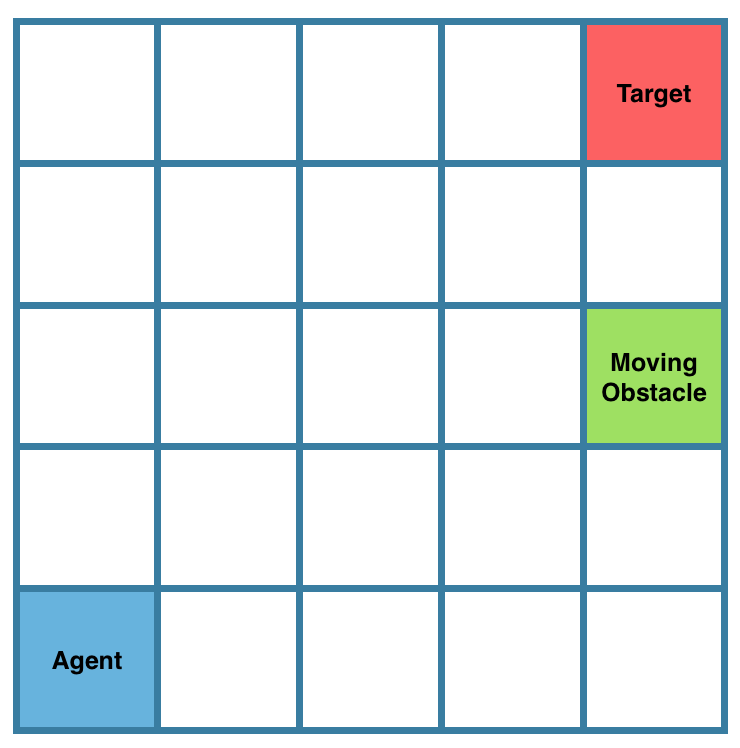
\includegraphics[width=0.5\columnwidth]{images/gridworld.png}
  \caption{Moving obstacle gridworld 	\label{fig:gridworld}}
\end{figure}
\begin{table}[]
\centering

\label{tab:results}
\begin{tabular}{|l|l|l|l|}
\hline
           & $\theta_e(\Phi_{a}-\Phi_{e)}$& $\theta_t(\Phi_{a}-\Phi_{t)}$ & $|\pi_a - \pi_t|$ (\%) \\ \hline
Original   & -6.125(2.06)        & 2.41(1.82)         & 15                    \\ \hline
Our Method & 0(0.2)              & 0.02(0.167)        & 10                    \\ \hline
\end{tabular}
\caption{Results on test set after 20 runs of random initial conditions. $\theta_e$ represent reward weights, $\pi$ represents policy and $\Phi$ represents feature expectations. The subscripts $a,e,t$ represent the apprentice, expert and taboo agents respectively. \jm{This table needs to be cleaned up. Try to keep the same number of significant figures in all entries.}}
\end{table}
It should be apparent from the results, \sw{These results show...} that using the additional data of avoidable behaviour \sw{don't use new words for concepts you've already introducted} allows the apprentice to 
come closer to the actual desired behaviour, which is that of the expert. Furthermore, in the third row of Table .. we can see that
even if the apprentice is trained only on the taboo agent, his policy and performance still come closer to the expert \sw{than what?}. This is further
evidence that learning to imitate and learning to avoid behaviours are related concepts and should be used interchangeable depending on the application. \sw{I don't understand this claim.}

\begin{figure}[t]
  \centering
  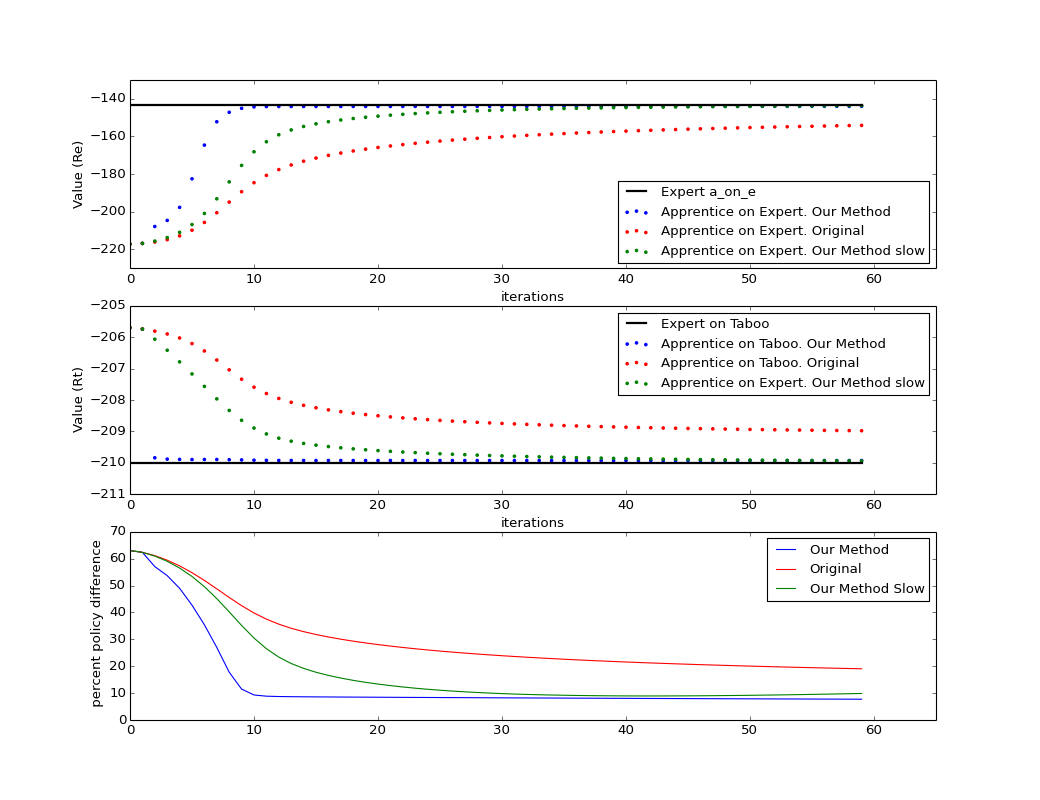
\includegraphics[width=0.9\columnwidth]{images/testgraph}
  \caption{A typical run for moving obstacle gridworld. Our method (blue) will quickly outperform the original algorithm. Achieving value that is closer to that of the expert, and reducing the difference with the desired policy\label{fig:results}}
\end{figure}

\subsection{Real Social Navigation Data.}




\section{Related Work}

\sw{Given that space will be tight, this should just be folded into the rest of the paper: mention each ref when it is relevent, primarily in background, but also in method and experiments.}


\section{Conclusions and Future Work}

\sw{This can be modeled on the new abstract once it's written.  We do need some future work ideas.} \jm{Perhaps we can mention further robot tests and validation of these results as future work. There was also this idea on the table of coupling this learning from failure approach with other IRL / LfD algorithms}

In this paper we have introduced a new framework for Inverse Reinforcement Learning that allows an agent to not only imitate certain behaviours but to also avoid others. The benefits this approach is that it allows otherwise useless data to be used and further enables a designer to inject prior information in the learning, by specifying, through simulated data, what behaviours should be avoided. We have derived a theoretically sound method by directly modifying the derivation of the Maximum Entropy and carrying that through to MaxEnt IRL, providing solutions to the computational obstacles that arise. We have further performed exhaustive experiments in a toy domain, that clearly demonstrate that our method can generalise much better that the baseline IRL algorithm. Finally we have performed learning on real data, again showing that our method is superior to the baseline.  

\bibliographystyle{aaai}
\bibliography{references}
	
\end{document}
